In this chapter, I present the theoretical background necessary to understand the modeling of globular clusters and stellar streams performed in this thesis. Much of the content draws from two comprehensive introductions to galactic dynamics: Galactic Dynamics by Binney and Tremaine, and Galaxiesbook.org by Bovy. These references provide a solid foundation for the physics and mathematical tools used throughout this work.

A common assumption in galactic dynamics is the so-called fluid limit, in which the orbit of a star is determined by the smooth gravitational potential generated by the galaxy as a whole. In this approximation, interactions between individual stars are negligible. This assumption holds well in many contexts—but not in all.

Globular clusters are a notable exception. Their relatively small number of stars makes them too “grainy” for the fluid approximation to hold, yet they contain far too many stars to be treated as simple few-body systems. This intermediate regime is the subject of the aptly named Million Body Problem, explored in detail by Heggie and Hut. Their textbook provides a thorough survey of methods to address this challenge, and their preface offers an insightful summary of the central difficulty: globular clusters inhabit an awkward middle ground where neither the fluid limit nor simplified few-body interactions apply cleanly. As a result, no analytical theory fully captures their dynamics.

While this thesis focuses primarily on stellar streams—specifically, how stars escape from globular clusters and evolve under the influence of the galactic potential—it is important to acknowledge that the internal evolution of the progenitor clusters still affects the properties of the streams. Although the internal cluster dynamics lie outside the scope of this work, they place important constraints on the interpretation of our results.

The remainder of this chapter is structured to clarify the theoretical framework supporting this thesis. I divide the discussion into three main parts:

\begin{itemize}

    \item \textbf{Explicit physics} - the physical laws and initial conditions implemented in the simulations;



    \item \textbf{Implicit physics} - the emergent behavior of these systems, the assumptions involved, and the mathematical tools used to interpret the results;

    \item \textbf{Ignored physics} - relevant aspects of the problem that are beyond the scope of this thesis, but which impact the interpretation of our results. Where appropriate, I cite works that pursue these directions and discuss how future work could incorporate them to improve upon the current modeling.


\end{itemize}




\section{The Explicit Physics}
    My simulations solve the \textit{restricted three body problem}. In essence
    \begin{figure}
        \centering
        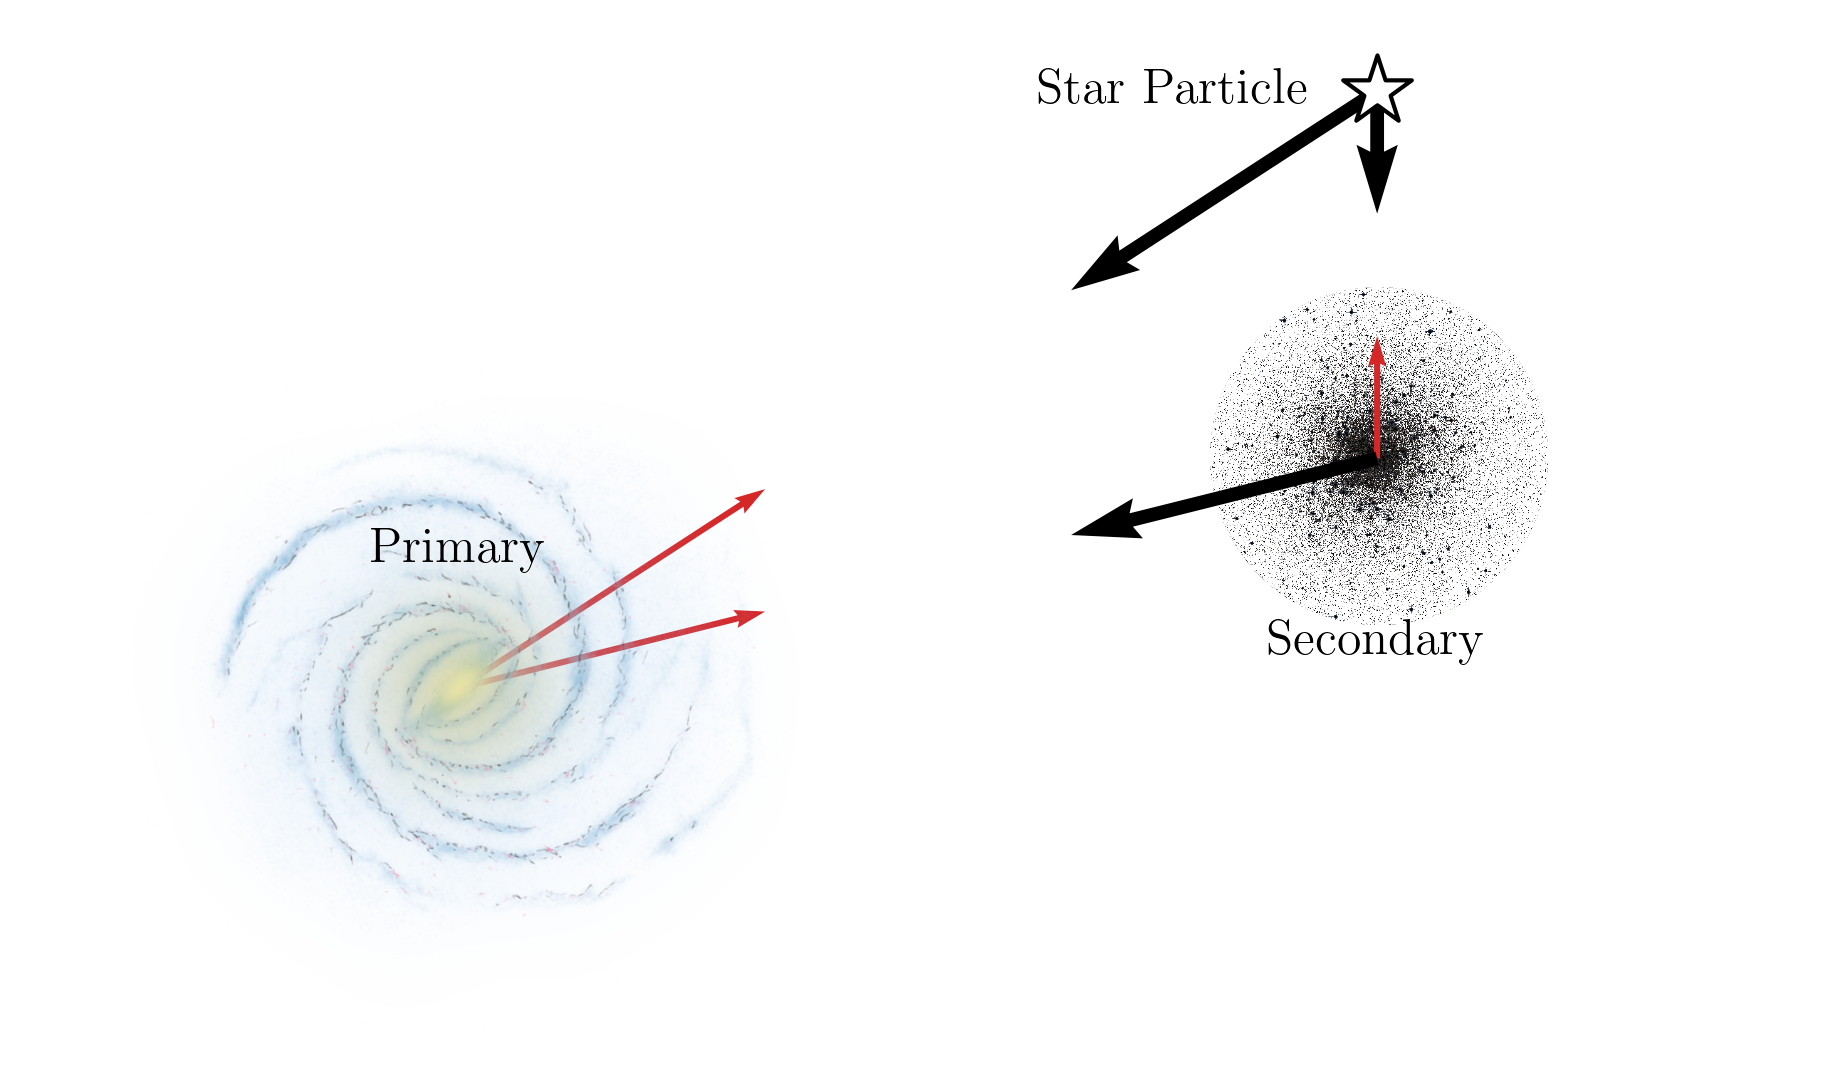
\includegraphics[width=\linewidth]{images/restricted_three_body_set_up.png}
        \caption{Little sketch of my equations of motion. }
    \end{figure}
    
    \subsection{Equations of Motion} \label{subsec:myEquationsOfMotion}
        I like to start with the \textit{Lagrangian}, which comes from the variational principle which states that particles with move along trajectories that minimize the difference, $ L = T-U $, which $L$ is the Lagrangian, $T$ is the kinetic energy and $U$ is the potential energy. Also, as is almost always the case in gravitational dynamics, we normalize by the mass and use \textit{specific} energy: 
        \begin{equation}
            \mathcal{L} = \frac{L}{m} = \frac{1}{2}\left(\dot{x}^2+\dot{y}^2+\dot{z}^2\right) - \Phi(x,y,z).
        \end{equation}
        However, Lagrange's equations give a system of three second order coupled ordinary differential equations. If we switch to Hamiltonain dynamics, we can object a set of six \textit{first} order ordinary differential equations, which is easier to implement computationally. Also, since we are using the specific energy, the momentum coordinates for Hamilton's equations are the same as the velocities from the Lagrangian: $ p_i = \frac{\partial \mathcal{L}}{\partial \dot{q}_i}$. Therefore, $p_i = \dot{q}_i$, where $i \in \left(x,y,z\right)$. The Hamilton is derived through the Legendre transform: $ \mathcal{H}=\sum_i p_i\dot{q}_i - \mathcal{L}$. Then, we can apply Hamilton's equations to obtain the set of equations: 
        \begin{align}
            \dot{p}_i &= -\frac{\partial \mathcal{H}}{\partial q_i} \\
            \dot{q}_i &= \frac{\partial \mathcal{H}}{\partial p_i}
        \end{align}

        And when written explicity become: 
        \begin{align}
            \dot{p}_x &= -\frac{\partial \Phi}{\partial x} \\
            \dot{p}_y &= -\frac{\partial \Phi}{\partial y} \\
            \dot{p}_z &= -\frac{\partial \Phi}{\partial z} \\
            \dot{x} &= p_x \\ 
            \dot{y} &= p_y \\ 
            \dot{z} &= p_z \\ 
        \end{align}        


        \subsubsection*{The Globular Cluster}
            In the case of the Globular Clusters, they only feel the Galaxy. So their Hamiltonian becomes: 
            % \begin{equation}

            % \end{equation}

        \subsubsection*{The Star Particles}

    \subsection{Potential density pairs}

        \begin{figure}
            \centering
            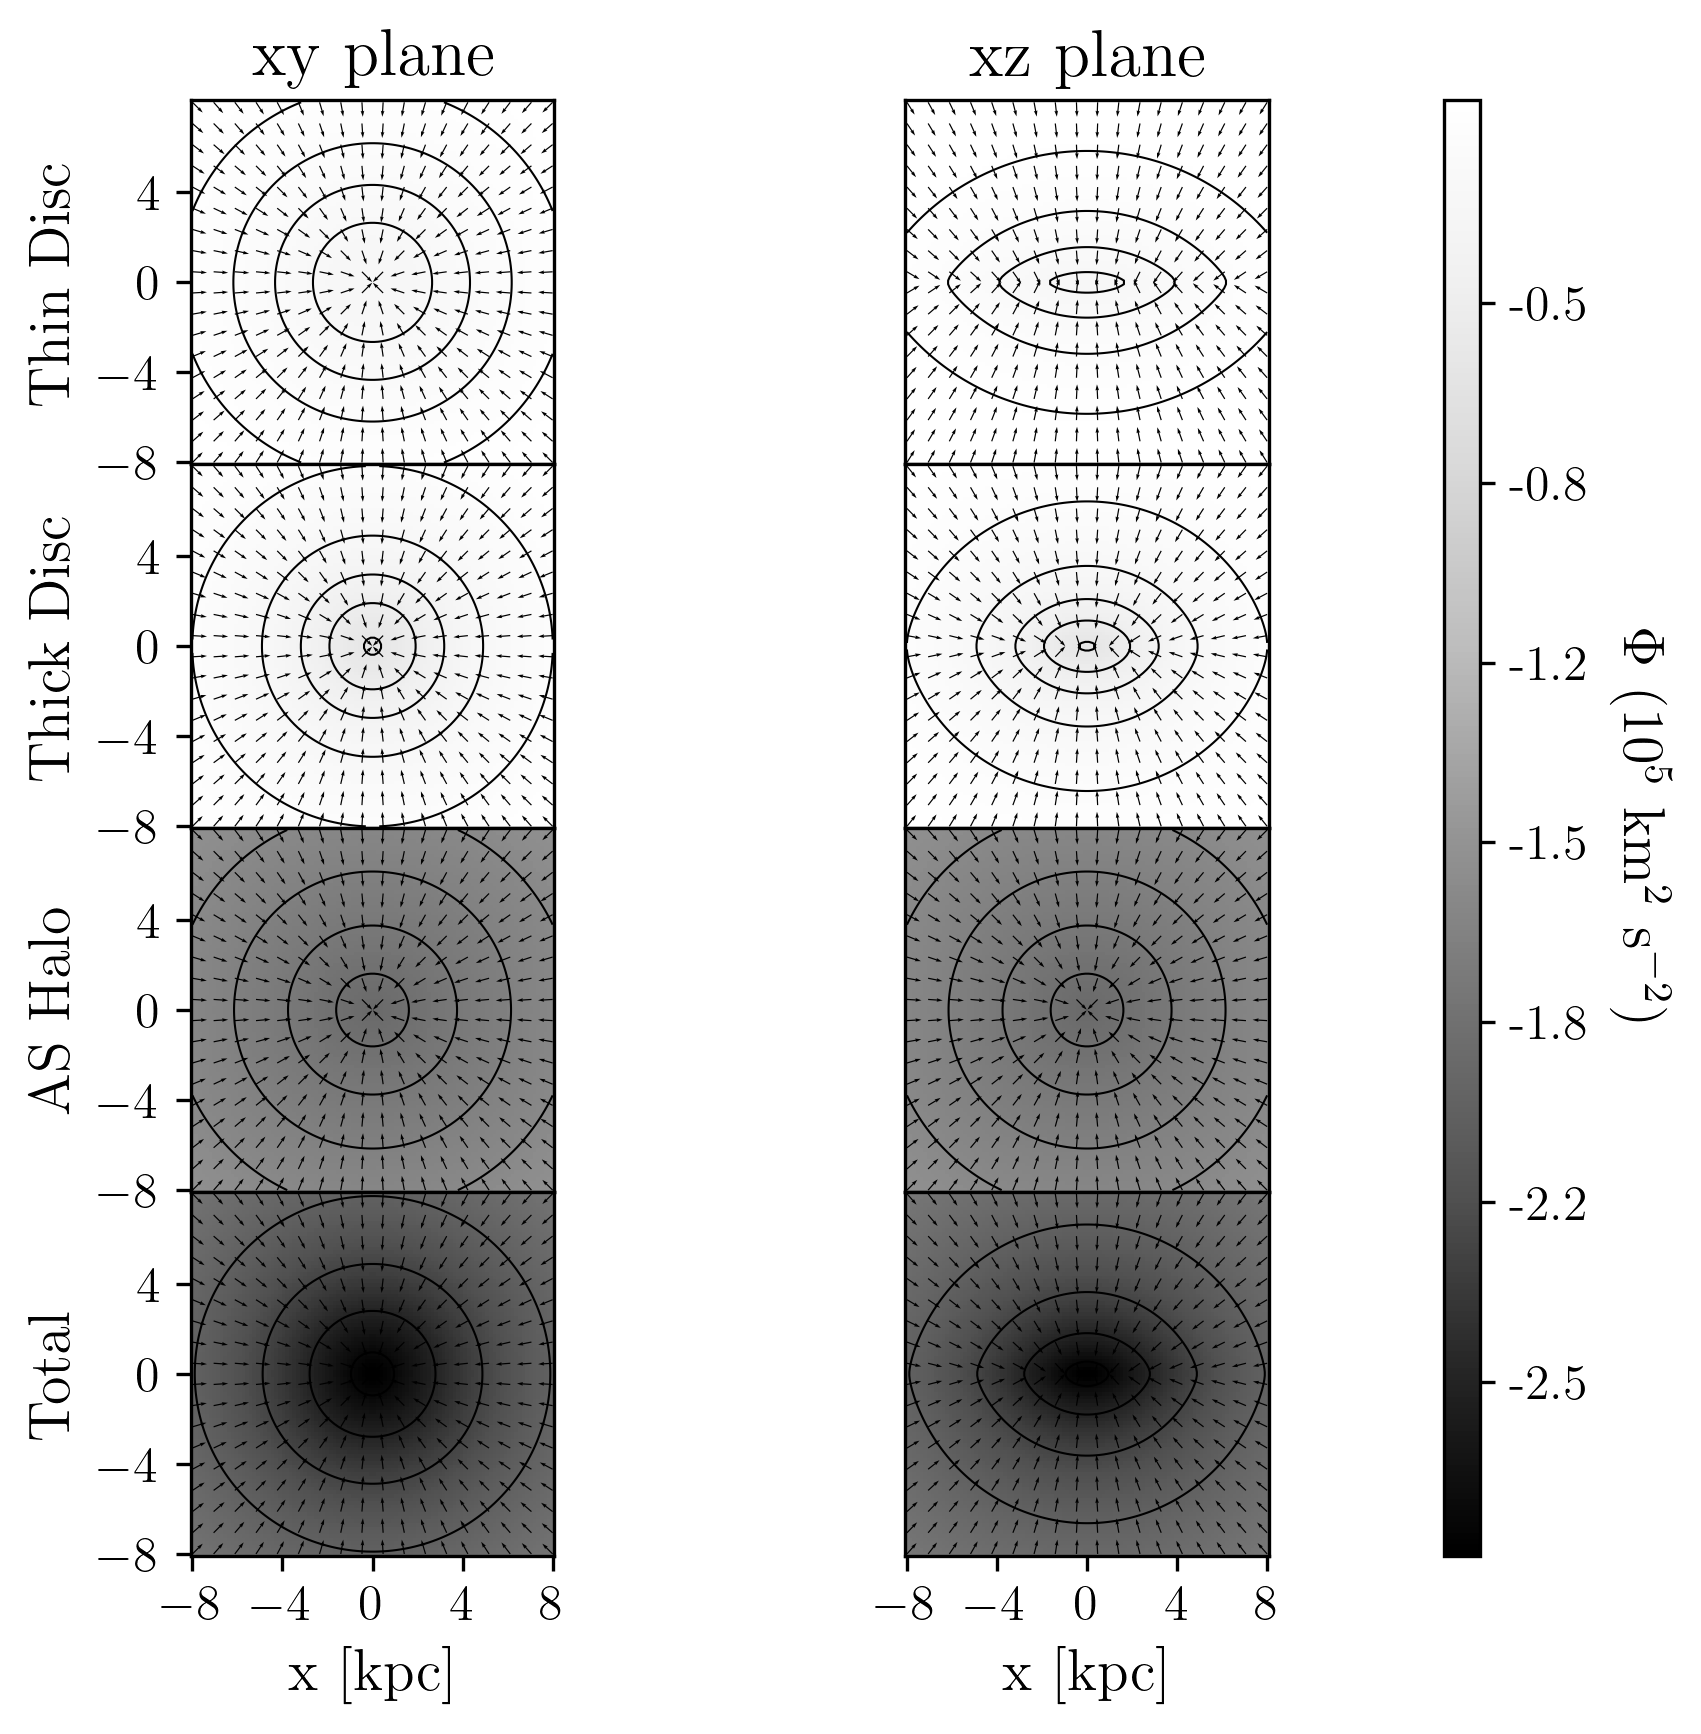
\includegraphics[width=\linewidth]{images/figure_pouliasis2017pii_potential_-8_8.png}
            \caption{The main potential used throughought the thesis}
        \end{figure}        
    

\section{The Implicit Physics}

    \subsection{The circular restricted three body problem}
        \begin{itemize}
            \item The Lagrange points
            \item Allowed regions 
        \end{itemize}

    \subsection{The tidal tensor}
        \begin{itemize}
            \item Either the Hessian of the Potential
            \item Or the Jacobian of the transform from position to force
            \item I prefer Jacobian
            \item We always use cartesian coordinates because if you do other systems, such as cylindrical or spherical, then you need to compute the cristoffer symbols. 
            \item Positive eigen values is stretching
            \item Negative eivenvalues is compression
            \item Stetching is a stronger deformation than compression
            \item For a spherical potential, the stretching deformation is parallel to the position vector. 
        \end{itemize}
        
        \begin{equation}
            \text{J}(F)= \left(\begin{matrix}
                \partial_x F_x & \partial_y F_x & \partial_z F_x \\
                \partial_x F_y & \partial_y F_y & \partial_z F_y \\
                \partial_x F_z & \partial_y F_z & \partial_z F_z 
            \end{matrix}\right)
        \end{equation}
        
        \subsubsection*{The Moon}


            \begin{itemize}
                \item If you talk about the tides, you have to start the conversation with the moon
                \item Cite the NASA website and say how many different ways we can evoke the tides
                \item since I do dynamics, I will discuss how the tides effect the orbit of the moon. 
                \item show with this little film that the tides slow down the orbit of the moon, make its distance wobble, and if you ignore it and only solve the 2 body problem + a rotating reference frame, after about 3/4 years you'll be completely off about your prediction.
                \item This is a cool point because the tides are even relevant on human time scales 
                \item There is no darkside of the moon. 
                \item cite the initial conditions from JPL
                \item Note that the drift of the moon from the earth is actually caused by the ocean and not the sun. Kinda crazy.
                \item Say this model is also an over simplification and that there's a whole field of study dedicated to all the librations of the moon with all the \textit{pertubations} from the simple two body problem. 
            \end{itemize}

            The tidal tensor for a keplerian potential: 
            \begin{equation}
                \mathcal{T}_{i,j}= \frac{GM_\odot}{r^3}\left(\begin{matrix}
                    1-\frac{3x^2}{r^2} & -\frac{3xy}{r^2} & -\frac{3xz}{r^2} \\
                    -\frac{3yx}{r^2} & 1-\frac{3y^2}{r^2} & -\frac{3yz}{r^2} \\
                    -\frac{3zx}{r^2} & -\frac{3zy}{r^2} & 1-\frac{3z^2}{r^2}
                \end{matrix}\right)
            \end{equation}            
\begin{verbatim}
VIDEO: moon_tidal_simulation.mp4
\end{verbatim}

            \begin{figure}
                \centering
                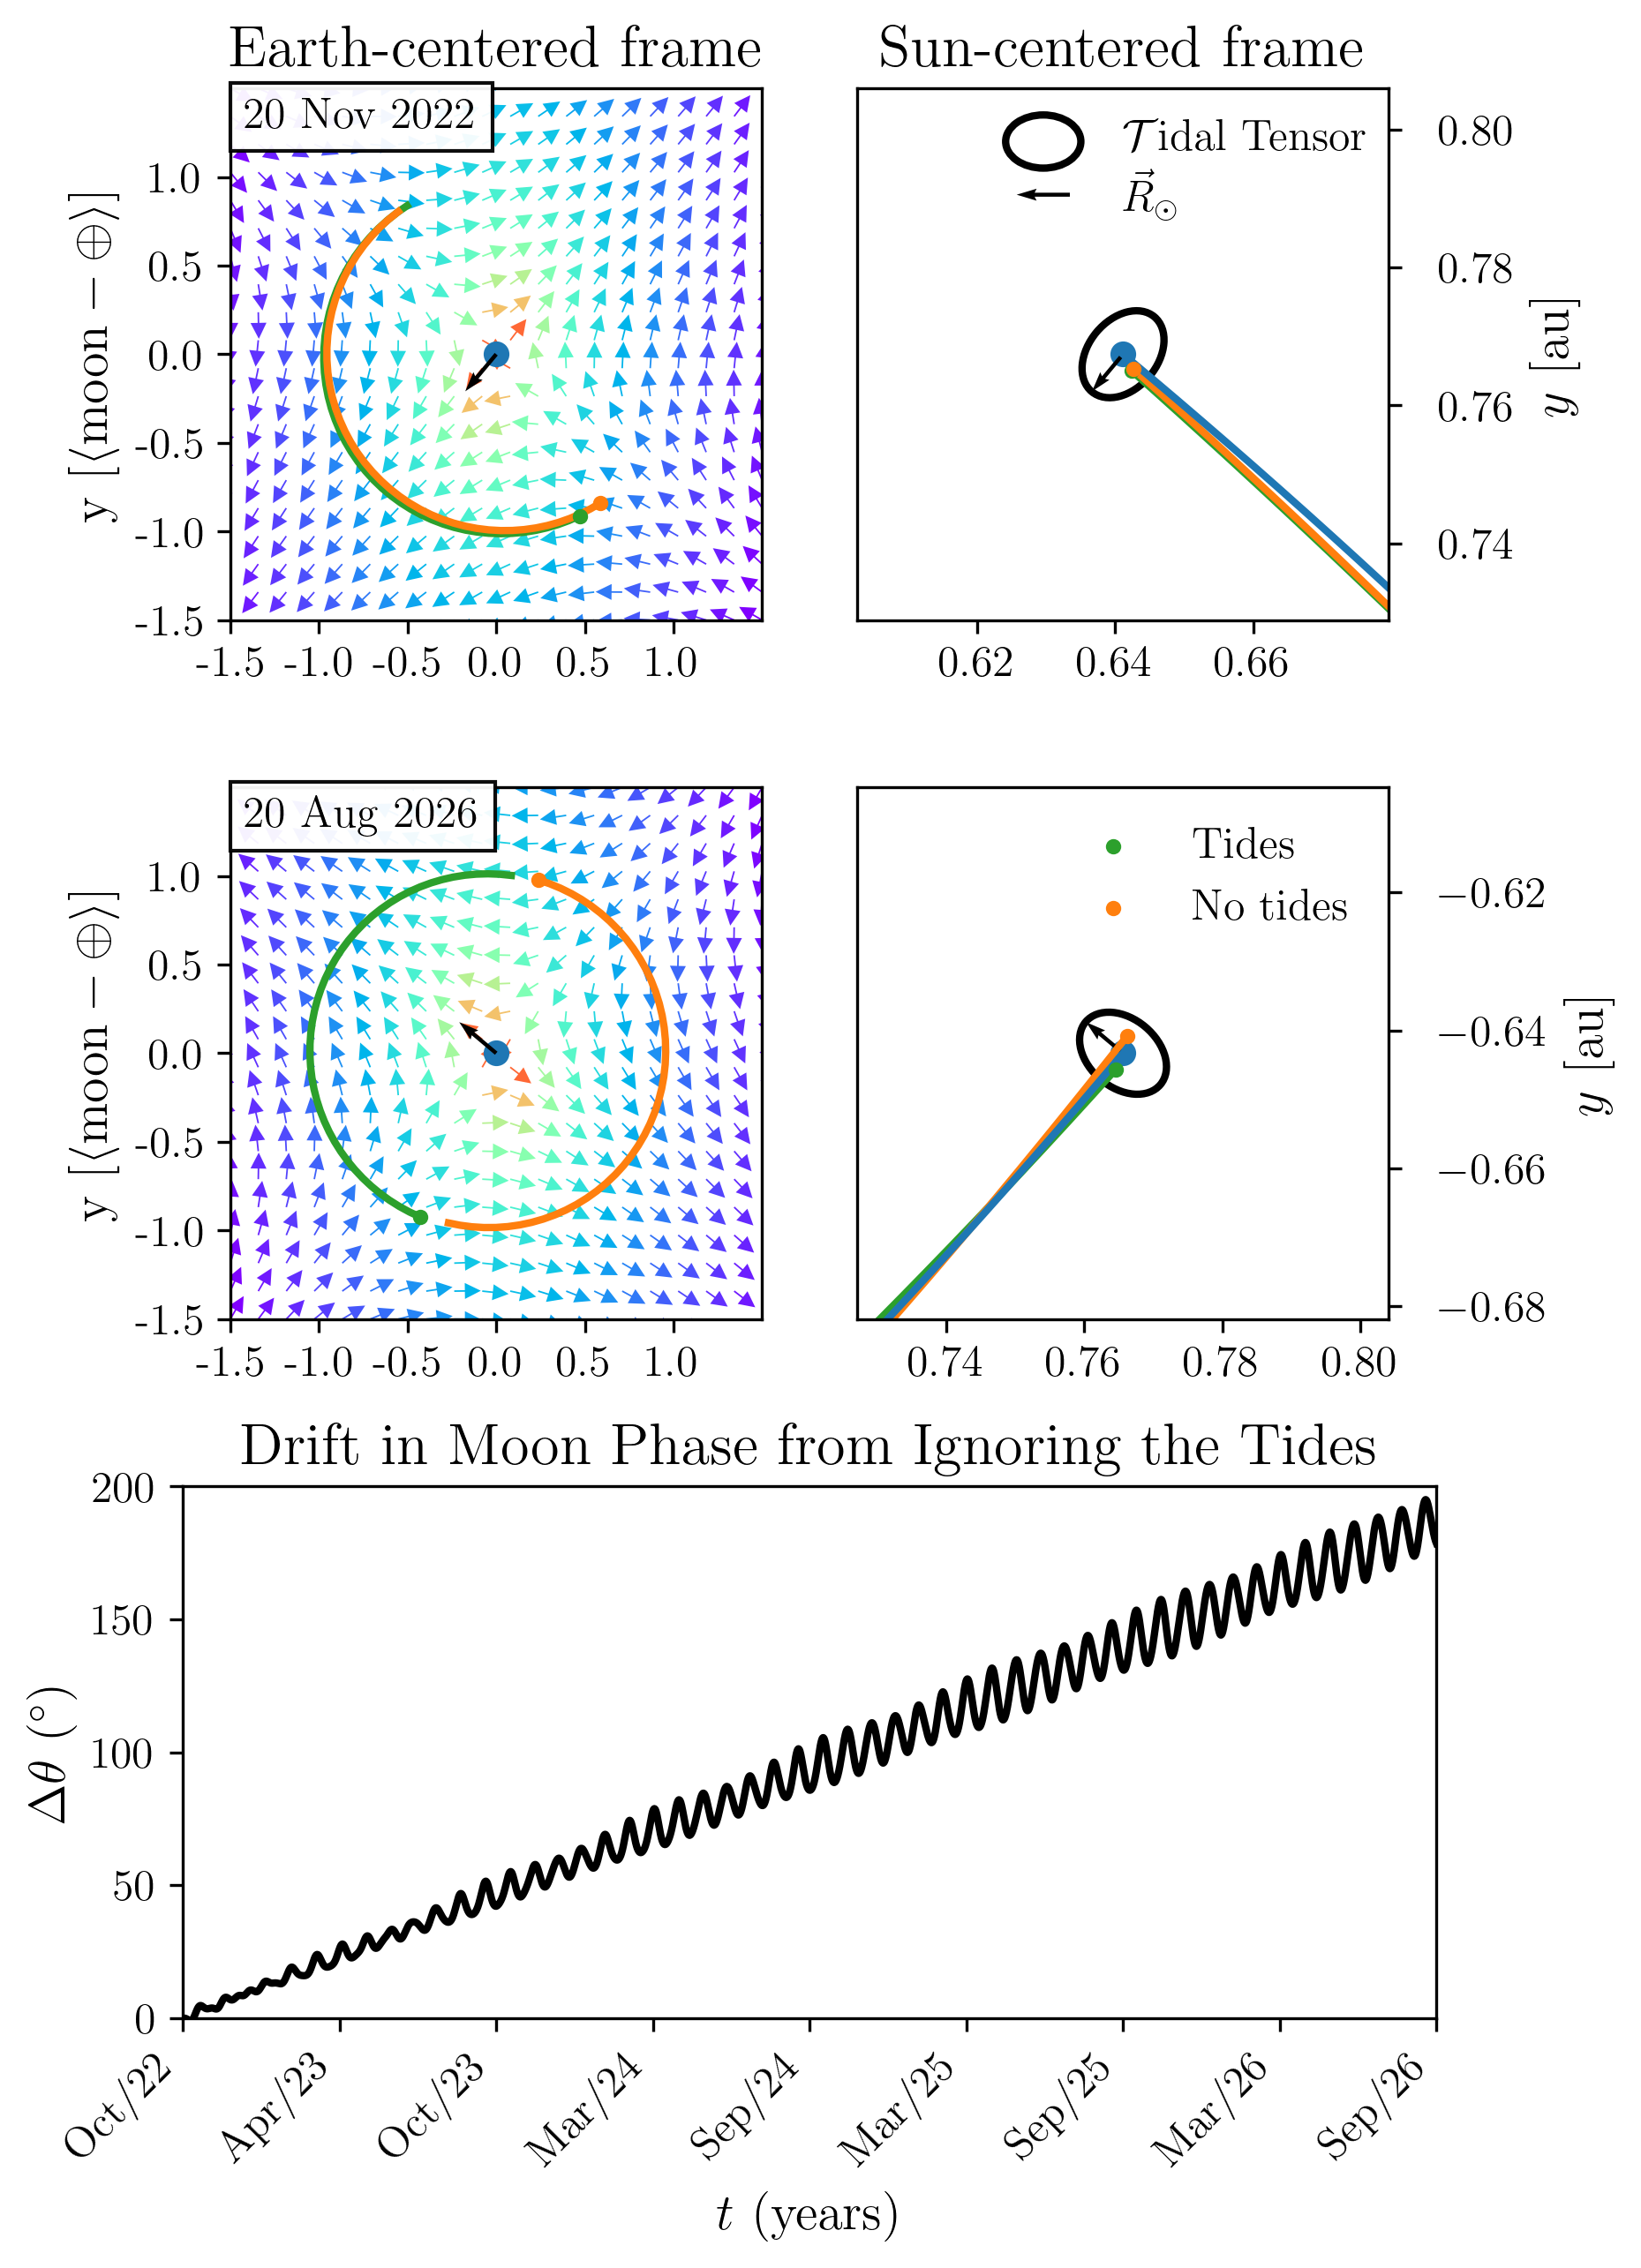
\includegraphics[width=\linewidth]{images/moon_tidal_simulation.png}
                \caption{The main potential used throughought the thesis}
            \end{figure}

        \subsubsection*{Tides in the Galaxy}
            \begin{itemize}
                \item Show some positions of the tidal tensor and how it can change orientation based on it's altitude 
                \item The tidal forces add together linearly, so show the Halo and the Disc example together. 
            \end{itemize}

            The Miyamoto Nagai potential is: 
            \begin{eqnarray}
                \Phi'   &= \frac{1}{D}\\
                D       &= \sqrt{x^2 + y^2 + \beta^2(z)}\\
                \beta(z)   &= 1 + \sqrt{z^2 + b^2}\\
                \beta'(z) &= \frac{z}{\sqrt{z^2 + b^2}}\\
                \beta''(z)  &= \frac{b^2}{\left(z^2 + b^2\right)^{3/2}}
            \end{eqnarray}

            The dimensionless tidal tensor then becomes: 


            \begin{figure}
                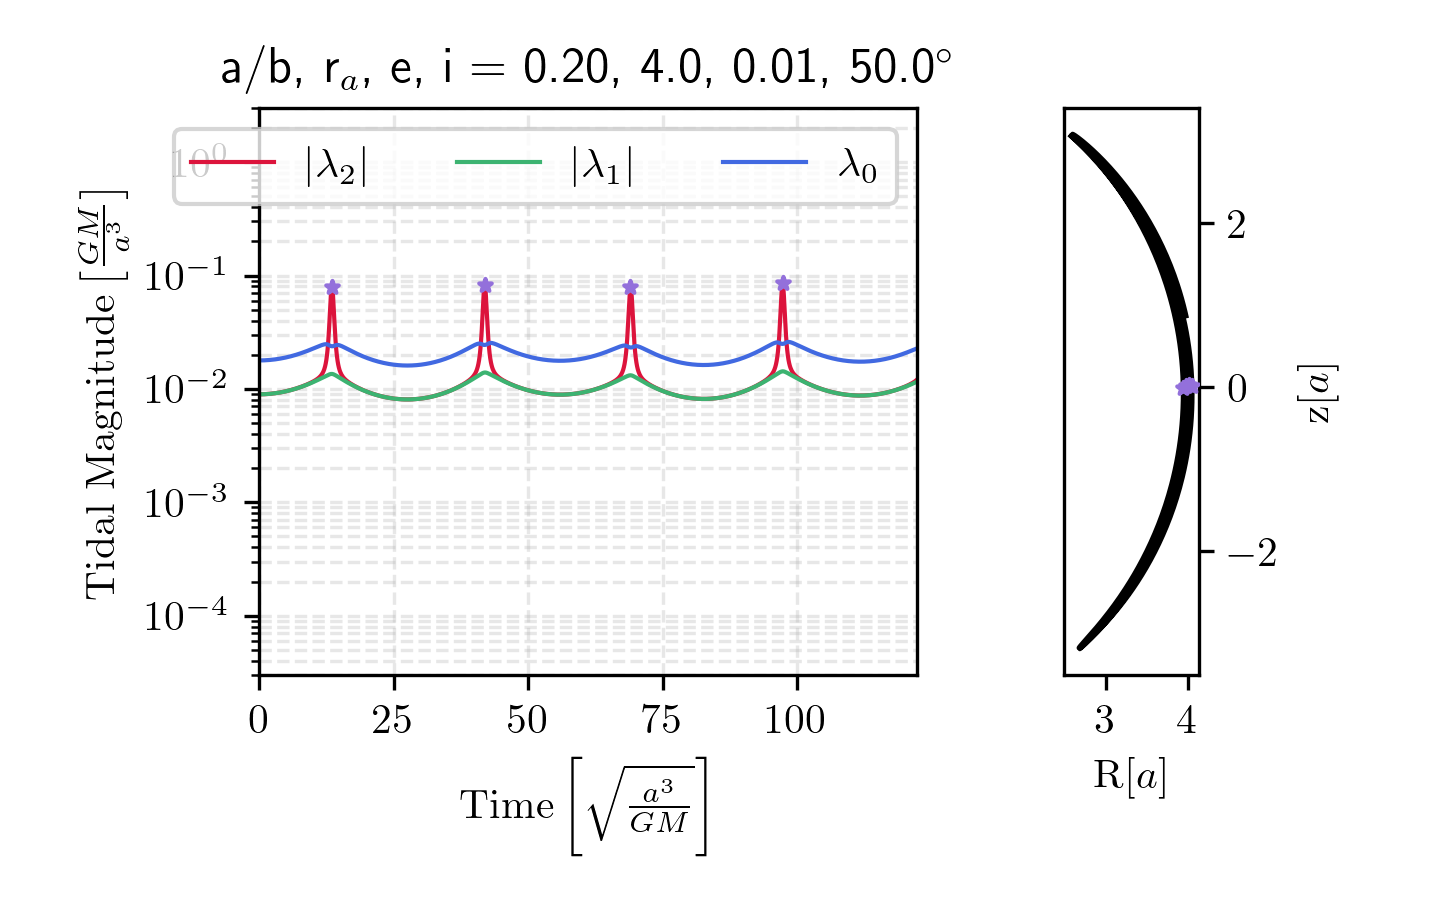
\includegraphics[width=\linewidth]{images/miyamoto_disc_shocks_ab_rp_e_i_0.20_4.0_0.01_50.0.png}
                \caption{No disk shocks on a planar orbit.}
                \label{fig:miyamoto_disc_shocks_circular_inclined_orbit}
            \end{figure}



            \begin{figure}
                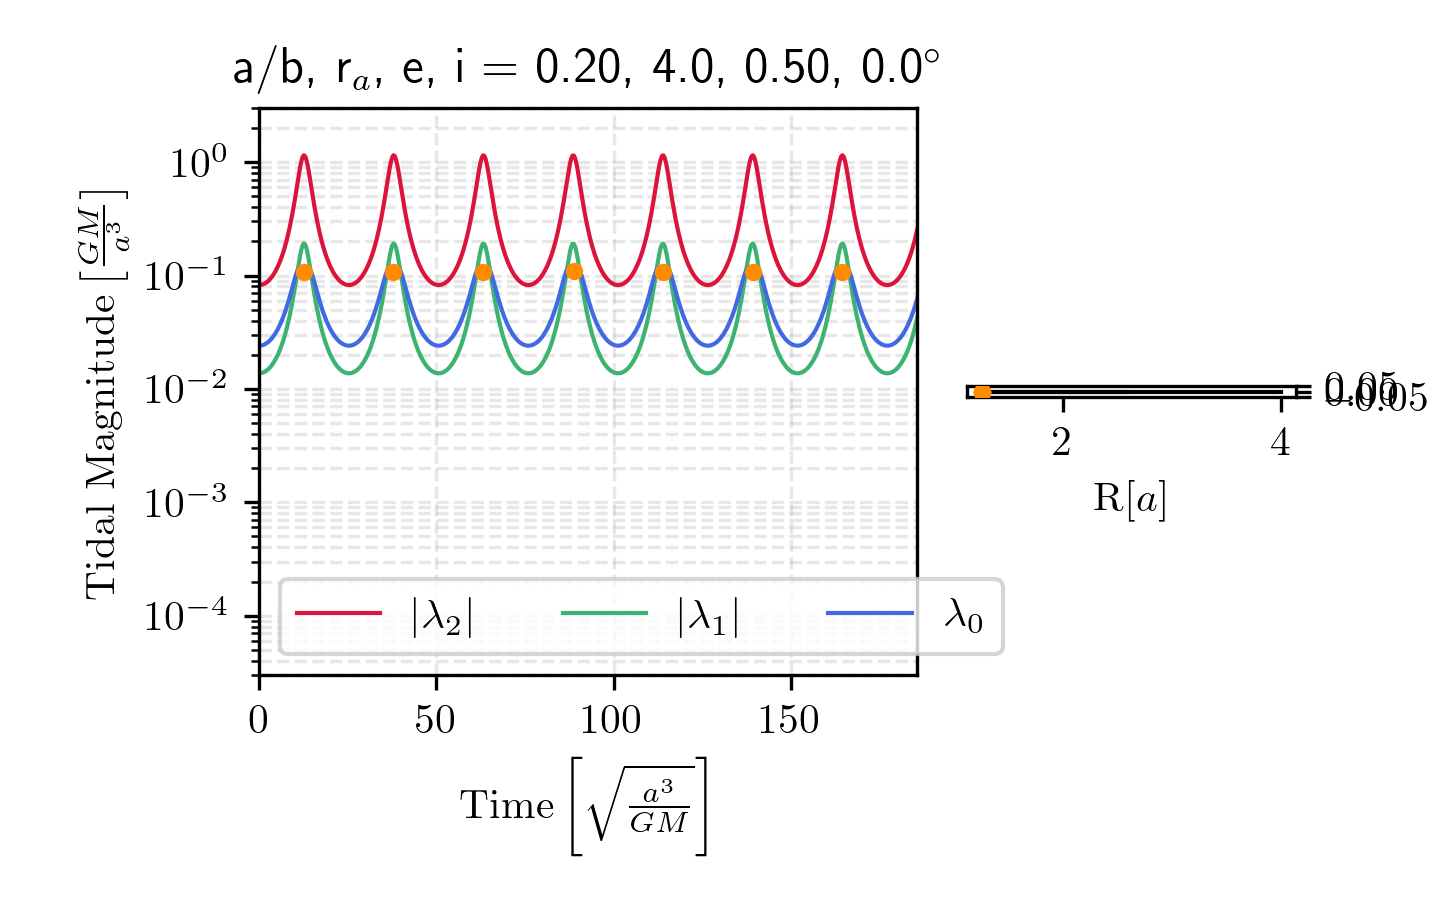
\includegraphics[width=\linewidth]{images/miyamoto_disc_shocks_ab_rp_e_i_0.20_4.0_0.50_0.0.png}
                \caption{Disk shocks on a circular inclined orbit.}
                \label{fig:miyamoto_disc_shocks_circular_inclined_orbit}
            \end{figure}

            \begin{figure}
                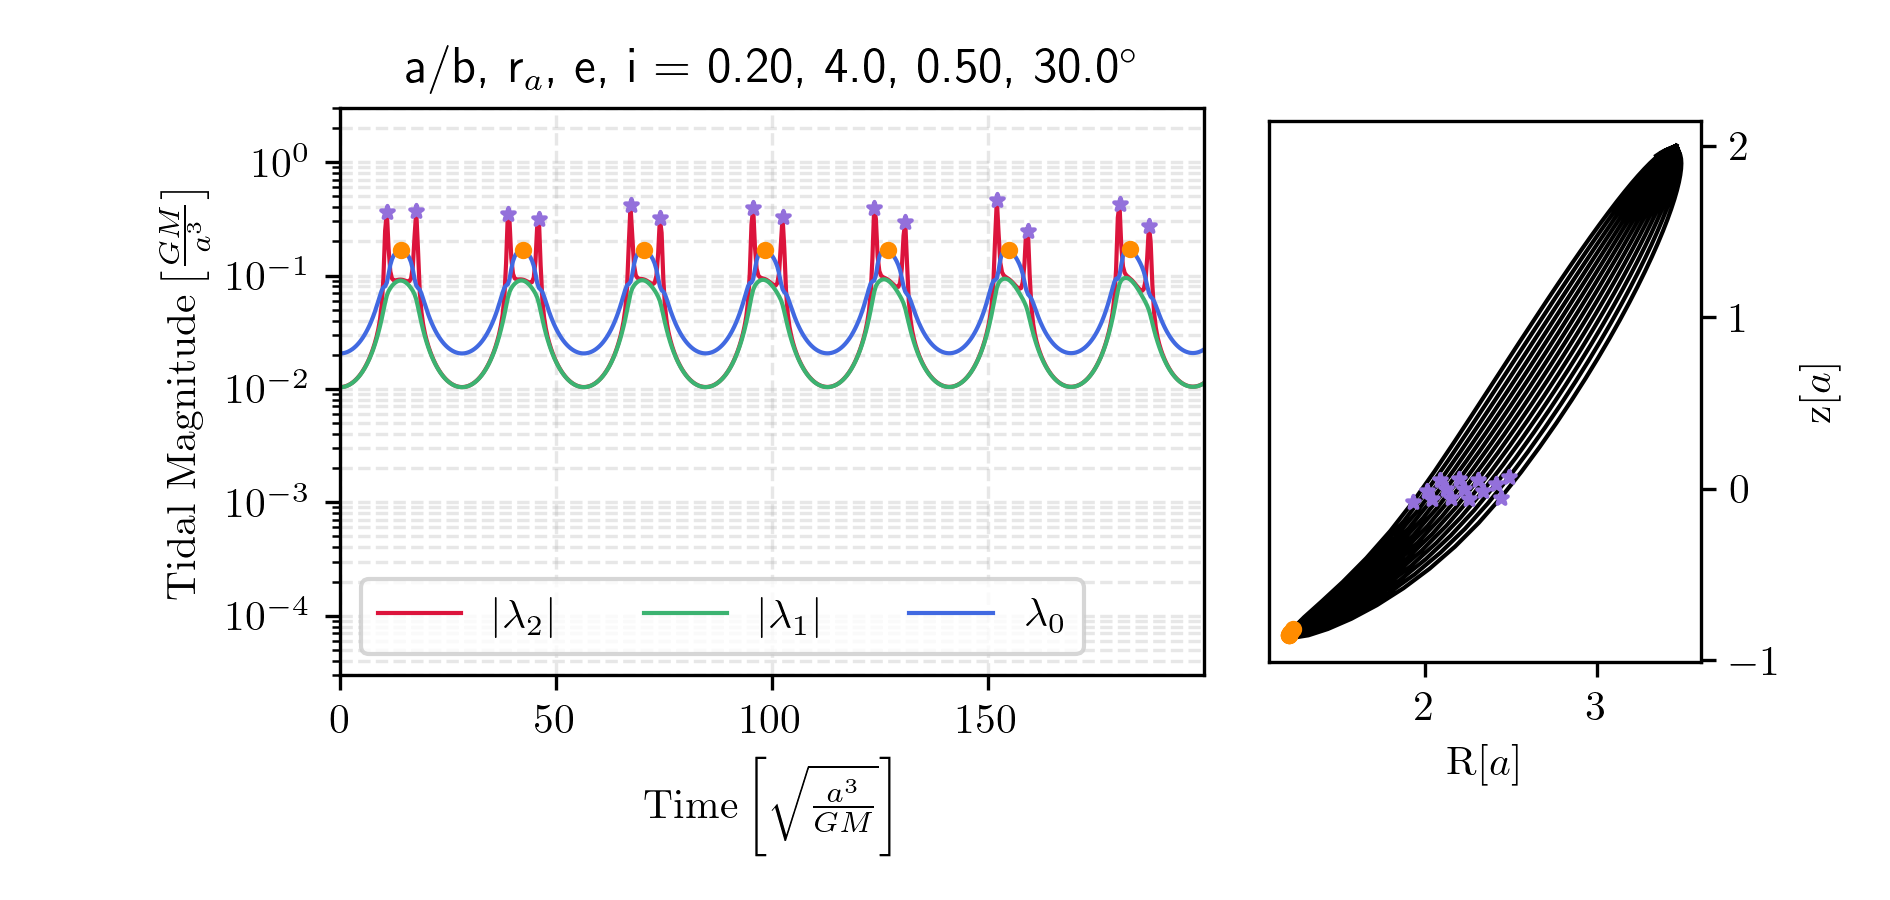
\includegraphics[width=\linewidth]{images/miyamoto_disc_shocks_ab_rp_e_i_0.20_4.0_0.50_30.0.png}
                \caption{Disk shocks on an orbit with resonant R and z.}
                \label{fig:miyamoto_disc_shocks_responant_R_z}
            \end{figure}
            
            \begin{figure}
                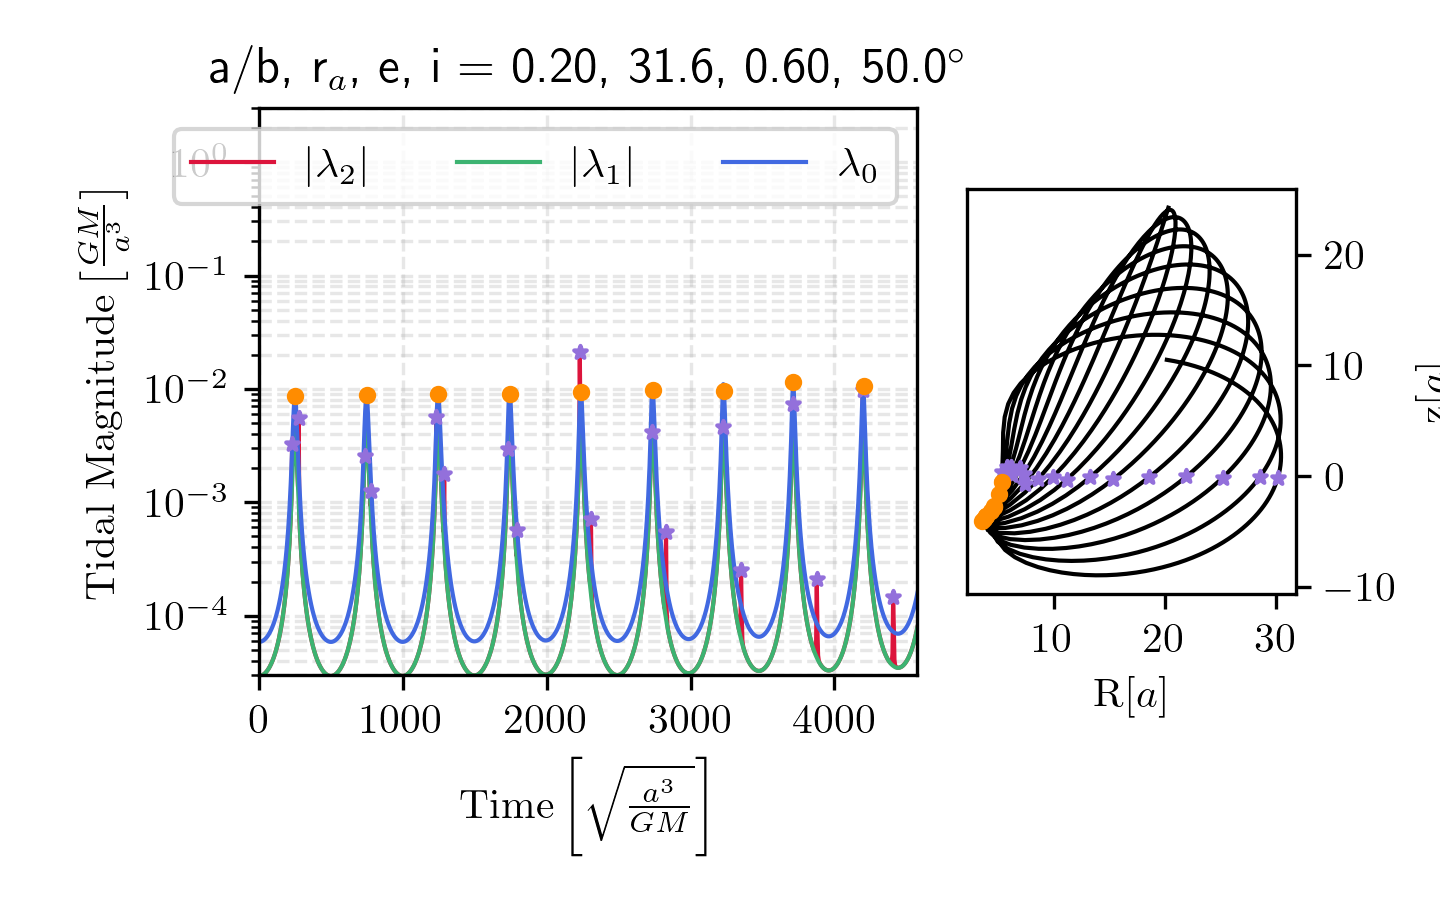
\includegraphics[width=\linewidth]{images/miyamoto_disc_shocks_ab_rp_e_i_0.20_31.6_0.60_50.0.png}
                \caption{Big apocenter}
                \label{fig:miyamoto_disc_shocks_big_apocenter}
            \end{figure}
            
            \begin{figure}
                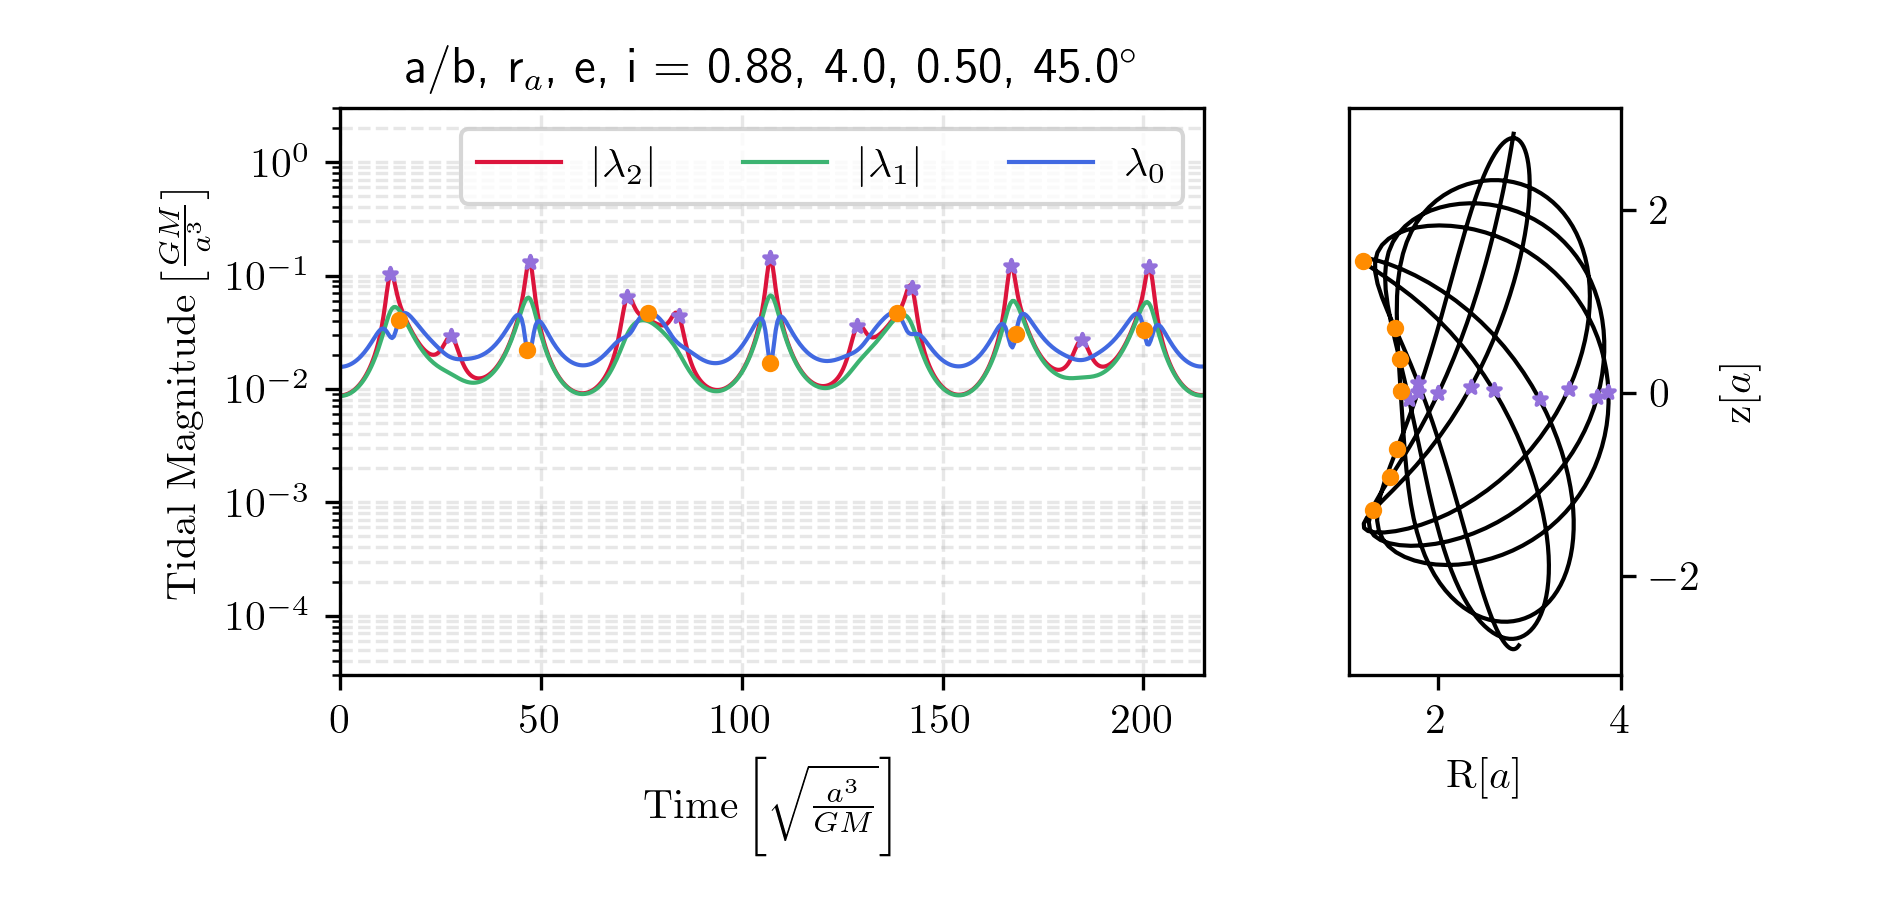
\includegraphics[width=\linewidth]{images/miyamoto_disc_shocks_ab_rp_e_i_0.88_4.0_0.50_45.0.png}
                \caption{Not very disky with this axis ratio}
                \label{fig:miyamoto_disc_shocks_weak_shocks}
            \end{figure}


            \begin{equation}
                \mathcal{T}_{i,j}=-\frac{1}{D^3}\left(\begin{matrix}
                    1-\frac{3x^2}{D^2} & -\frac{3xy}{D^2} & -\frac{3x\beta \beta'}{D^2} \\
                    \dots & 1-\frac{3y^2}{D^2} & -\frac{3y\beta \beta'}{D^2} \\
                    \dots & \dots & \beta'^2 + \beta \beta'' -\frac{3\left(\beta\beta'\right)^2}{D^2}
                \end{matrix}\right)
            \end{equation}    
            You can see immediately that multiplying the matrix by $\vec{v}=\lambda\left[x,y,z\right]$ does not return a vector that is parallel to the position vector, as it does for the spherical mass distribution. 

            The Marto's halo has this mass distribution:
            
            \begin{equation}
                M'_\text{enc}(s) = \frac{s^\gamma}{1+s^{\gamma-1}}
            \end{equation}
            The dimensionless tidal tensor is thus: 
            \begin{equation}
                \mathcal{T'}_{i,j}= -\frac{M'_\text{enc}(s)}{s^3}\left(\begin{matrix}
                    1-\frac{x^2}{s^2}f(s) & -\frac{xy}{s^2}f(s) & -\frac{xz}{s^2}f(s) \\
                    -\frac{yx}{s^2}f(s) & 1-\frac{y^2}{s^2}f(s) & -\frac{yz}{s^2}f(s) \\
                    -\frac{zx}{s^2}f(s) & -\frac{zy}{s^2}f(s) & 1-\frac{z^2}{s^2}f(s)
                \end{matrix}\right)
            \end{equation}  
            where 
            \begin{equation}\label{eq:martos_f_s}
                f(s) = 2-\frac{\gamma-1}{1+s^{\gamma-1}}
            \end{equation}

        \subsubsection*{Interesting case}
            There is an interesting area in the parameter space where the tidal forces would impede creating stellar streams instead of making them, as shown in Fig.~\ref{fig:martos_tidal_field_small_r}.

            Taking the Martos tidal tensor in Eq.~\ref{eq:martos_f_s}, we can see that for $\gamma > 3$ and $s \ll  1$, then $f(s)< 0$. Physically, this would be a sphere whose density increases with distance. This is not natural, as, in general, gravity sends the more massive objects towards the center. However, it's fun to indulge in this situation to learn some insight about the flexibility of tidal fields. The consequence of $f(s)< 0$ is that all terms in the tidal tensor are negative, which means that the force is compressive everywhere. Consequently, no stars escape from the cluster. 

            In Fig.~\ref{fig:martos_tidal_field_small_r}, I present a small experiment demonstrating the consequence of such a tidal force on a globular cluster, which is that no tidal stream forms. Briefly, I created a plummer sphere of $10^6$~M$_\odot$ and half mass radius 20~pc and evolved it in a Martos halo potential of mass parameter $10^{12}$~M$_\odot$ a characteristic radius of $30$~kpc. Each cluster was placed at the same initial conditions, a distance of 1/4 the scale radius from the center of the potential. The initial velocity was made perpendicular to the position vector with a speed of $(1-e)v_\textrm{c}$. This is a pseudo-eccentricity, which was added to have a non-circular orbit to demonstrate how the trajectories change in the two cases. The top panel uses a $\gamma$ of 2.02, which is the same value in the model where the halo was originally presented, and the value I employ in this thesis. Next, the bottom panel uses $\gamma$ of 4.5, which corresponds to a density profile where $\rho(r) \propto r^{1.5}$. 

            To get a feel for the strength of the tidal stretching and compression, I show a circle and the resulting ellipse after applying the tidal deformation. I computed the coordinates of the ellipse by adding $\vec{Ell} = \vec{C} + \frac{1}{2} t_\textrm{char}^2 \mathcal{T}\cdot \left(\vec{C} - \vec{r_o}\right)$. This way, force can be mapped to position space, and the strengths of the tidal forces can be seen visually. The characteristic time, $t_\textrm{char}$, was set to $\frac{1}{10} 2\pi r_\textrm{halo} / v_\textrm{c}$. 
            
            \begin{figure}
                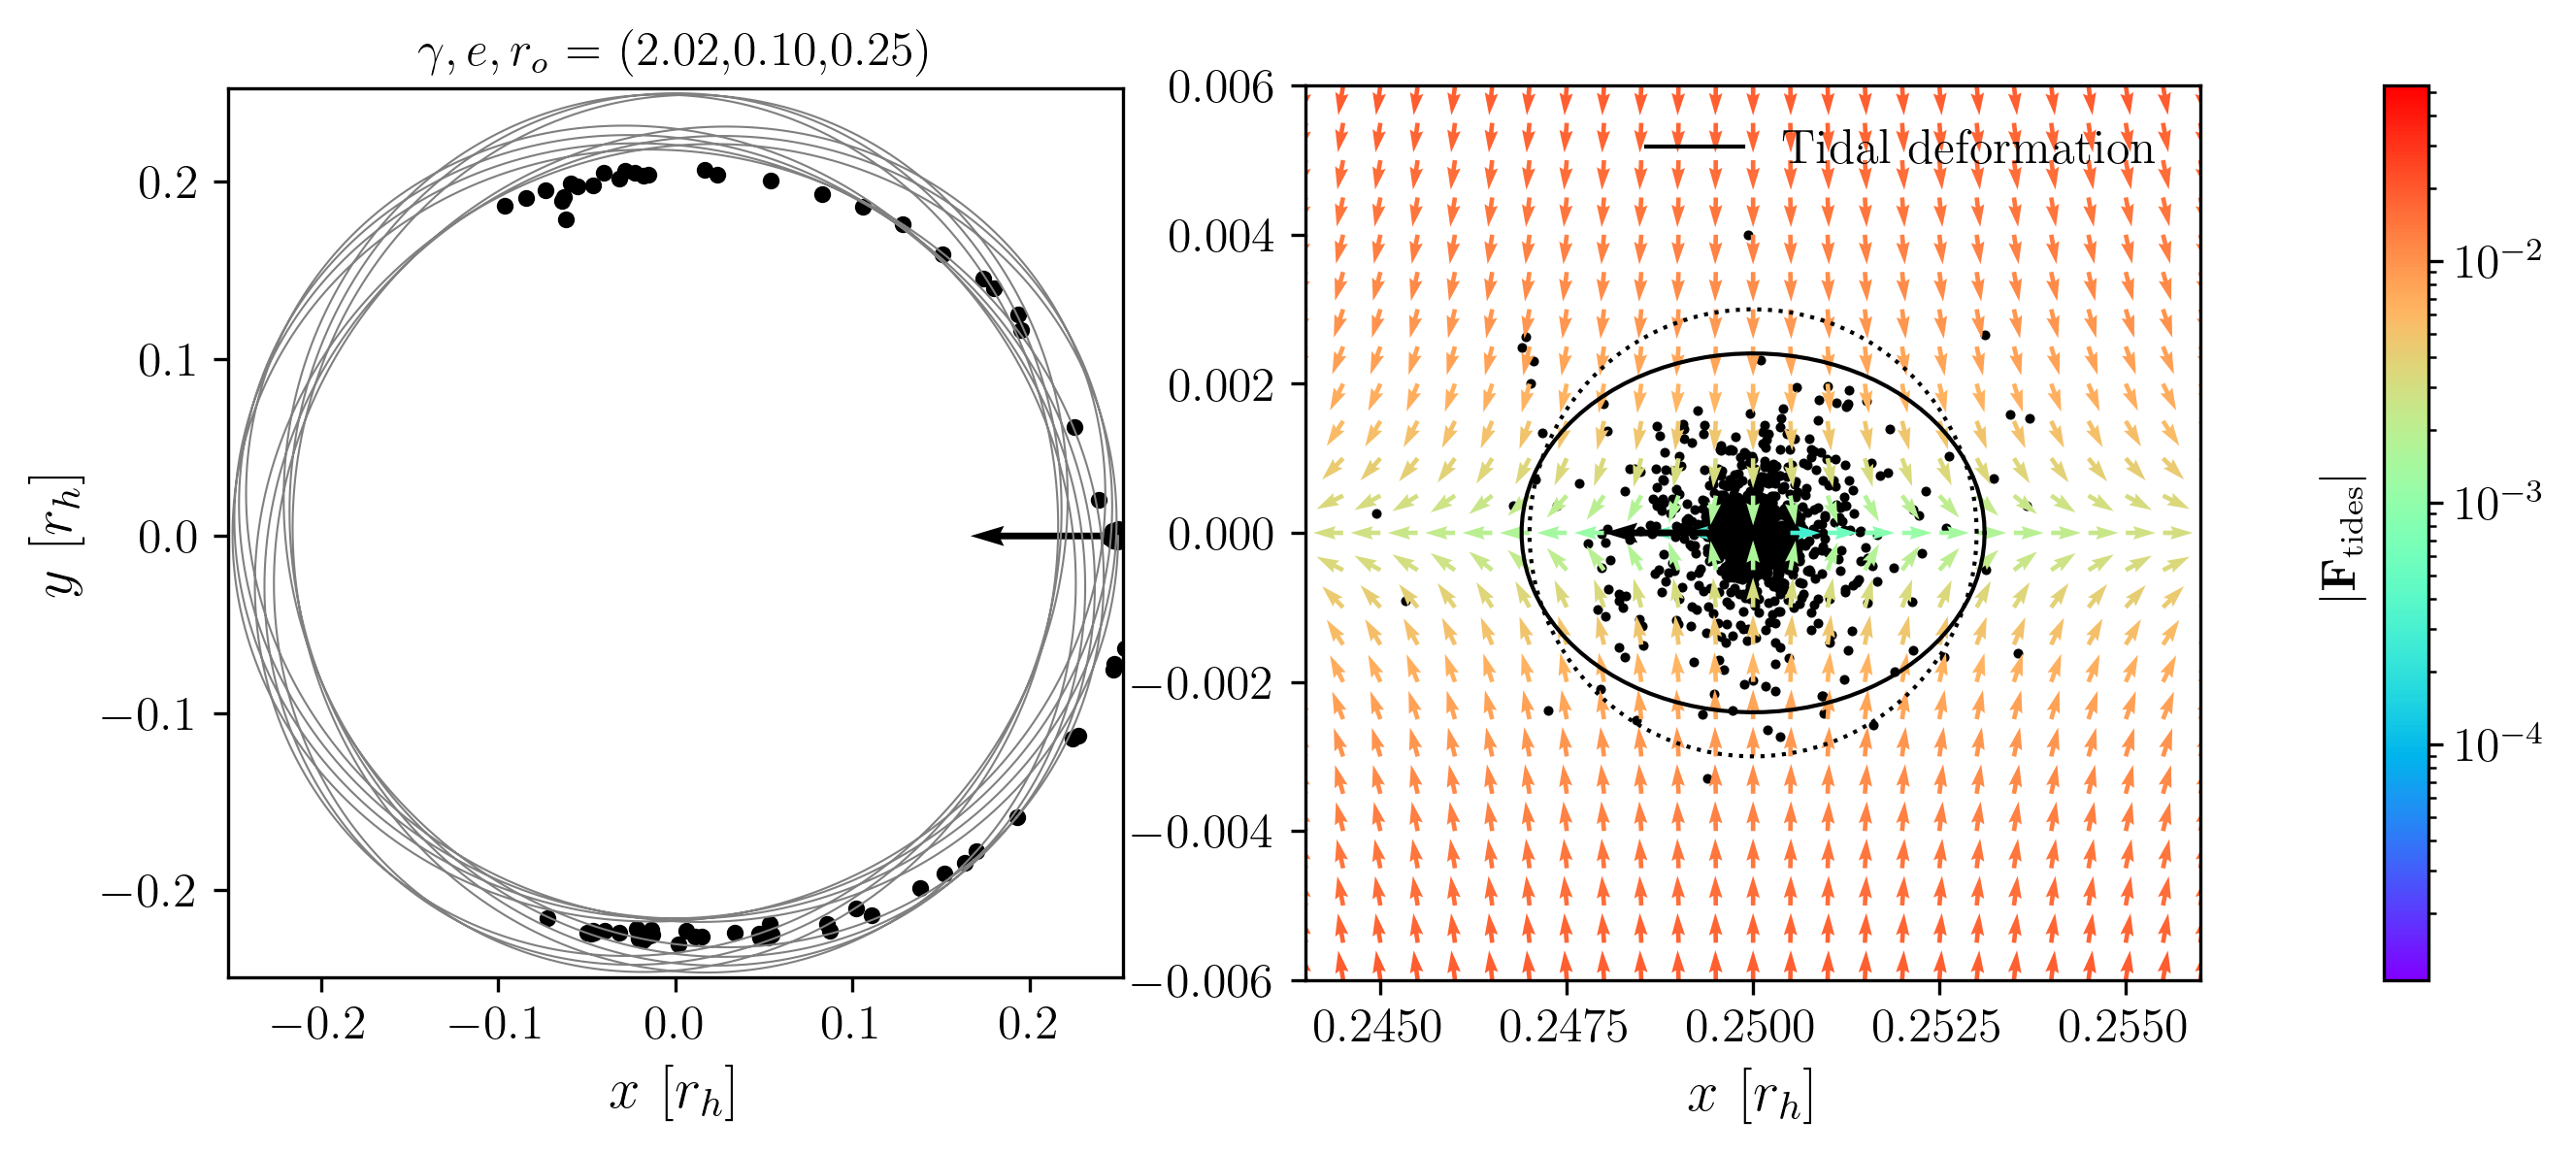
\includegraphics[width=\linewidth]{images/martos_tidal_field_202_10_25.png}
                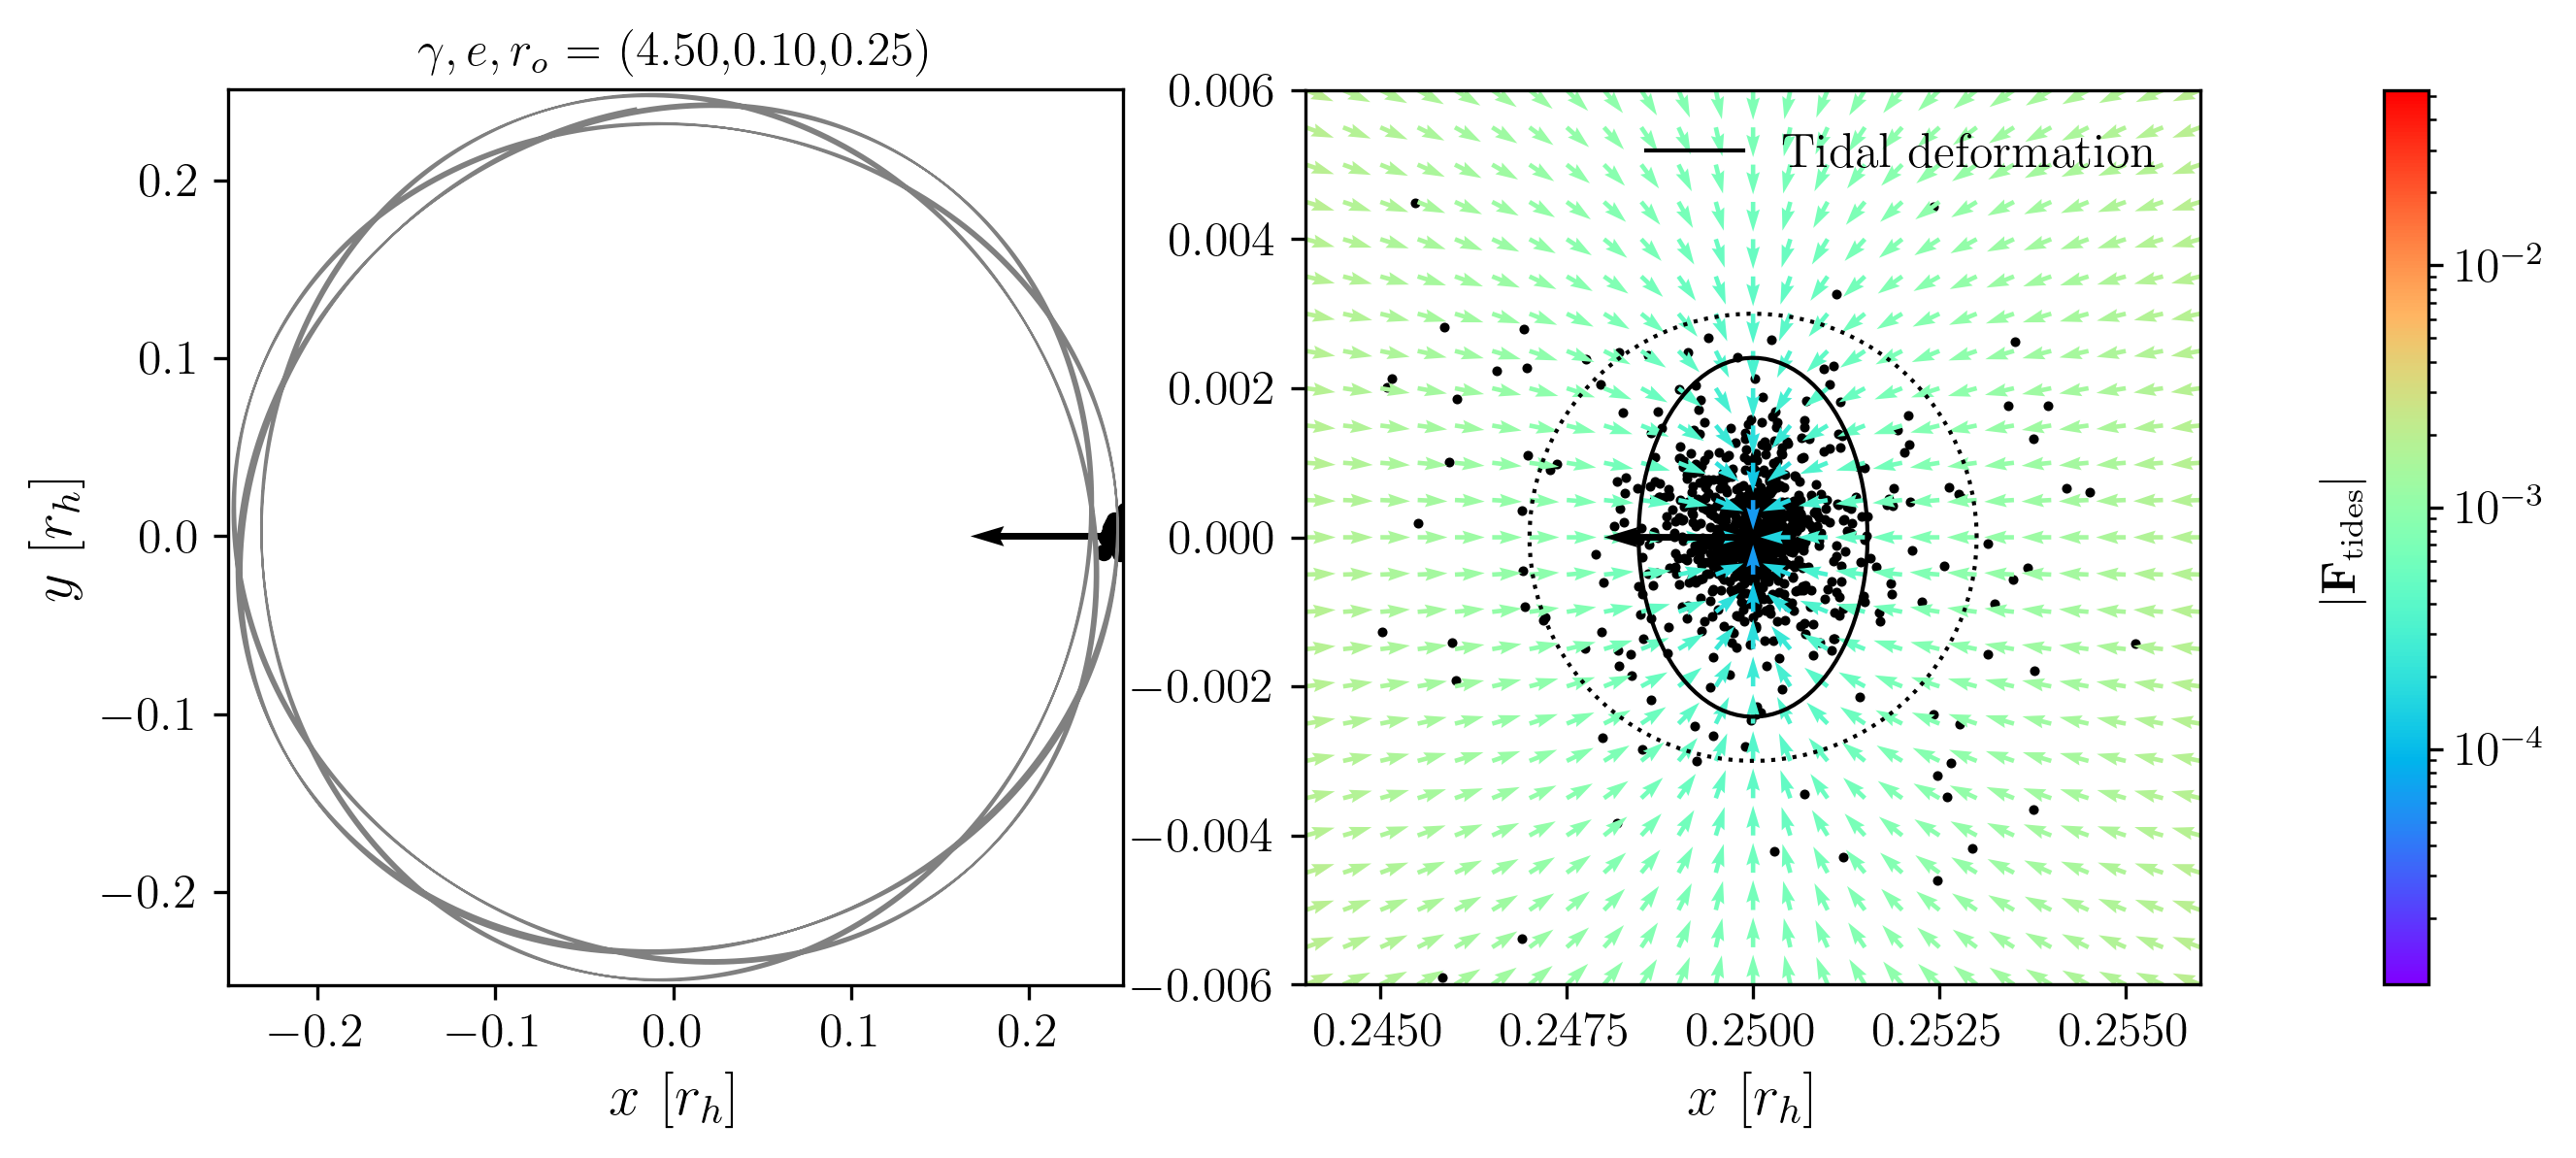
\includegraphics[width=\linewidth]{images/martos_tidal_field_450_10_25.png}
                \caption{The plots show two low-resolution streams (N = 1000) created by dissolving a Plummer sphere in the Martos halo potential. The units are scaled to the halo's characteristic radius. Gamma is the mass exponent and is the sole variable between the two simulations. The panels on the left show the orbit in gray and the stars in black. The black arrow points towards the center of the potential. The panels on the right show the tidal field, which is the tidal tensor evaluated at each position in space. The gray dotted circle is plotted with an arbitrary radius and is deformed by the tidal field into a black ellipse.}
                \label{fig:martos_tidal_field_small_r}
            \end{figure}

            \begin{figure}
                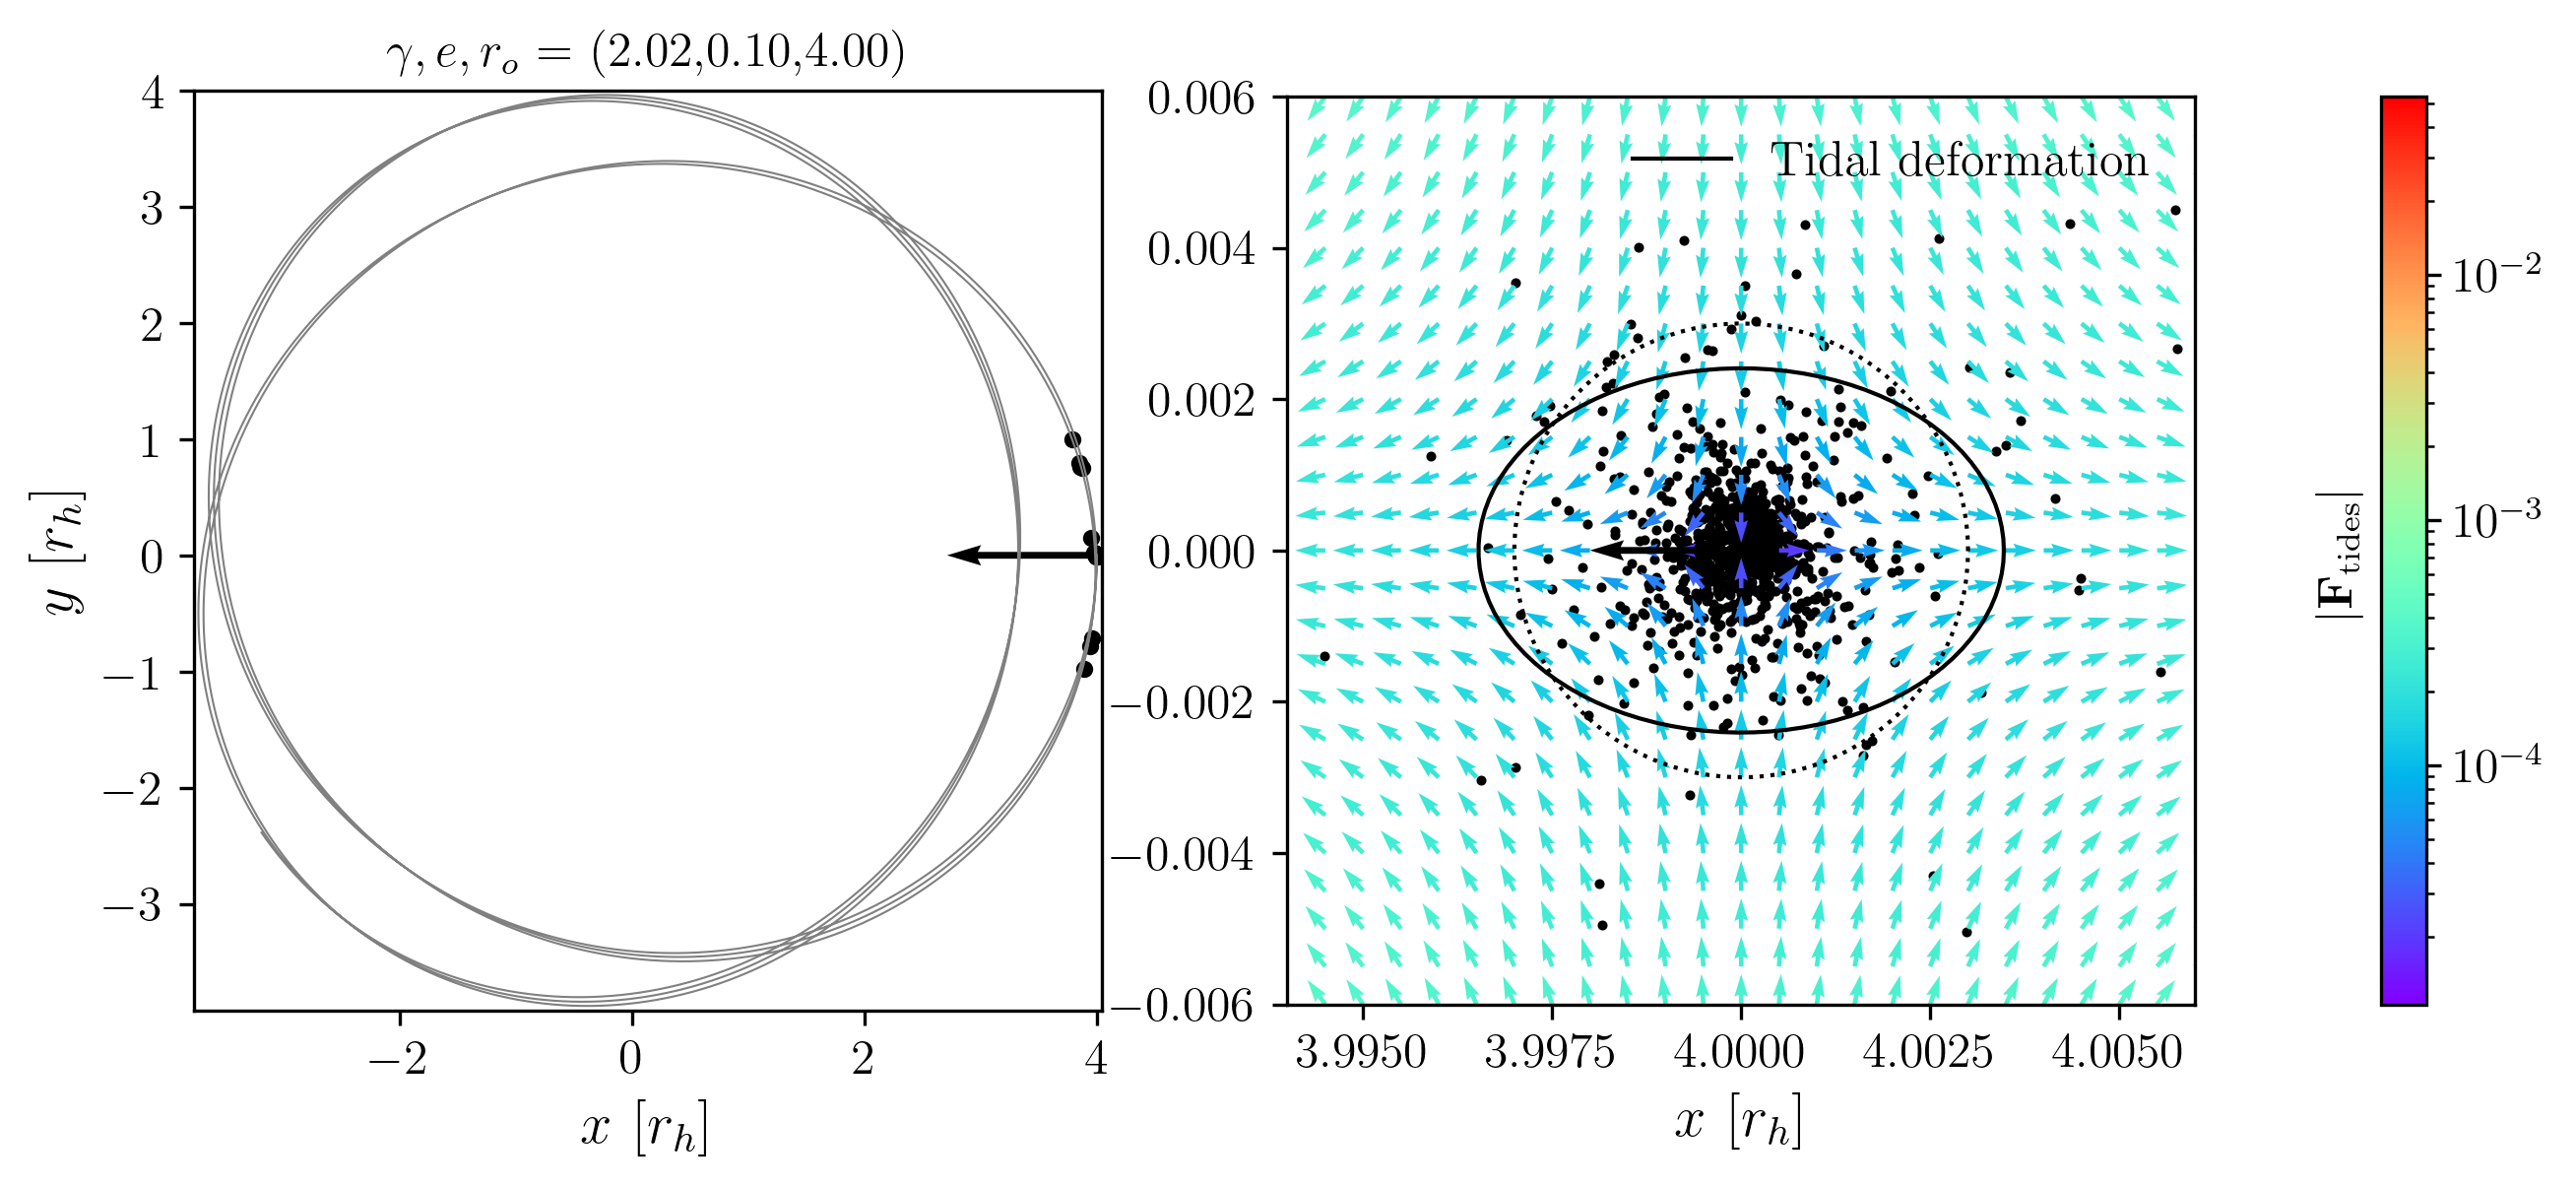
\includegraphics[width=\linewidth]{images/martos_tidal_field_202_10_400.png}
                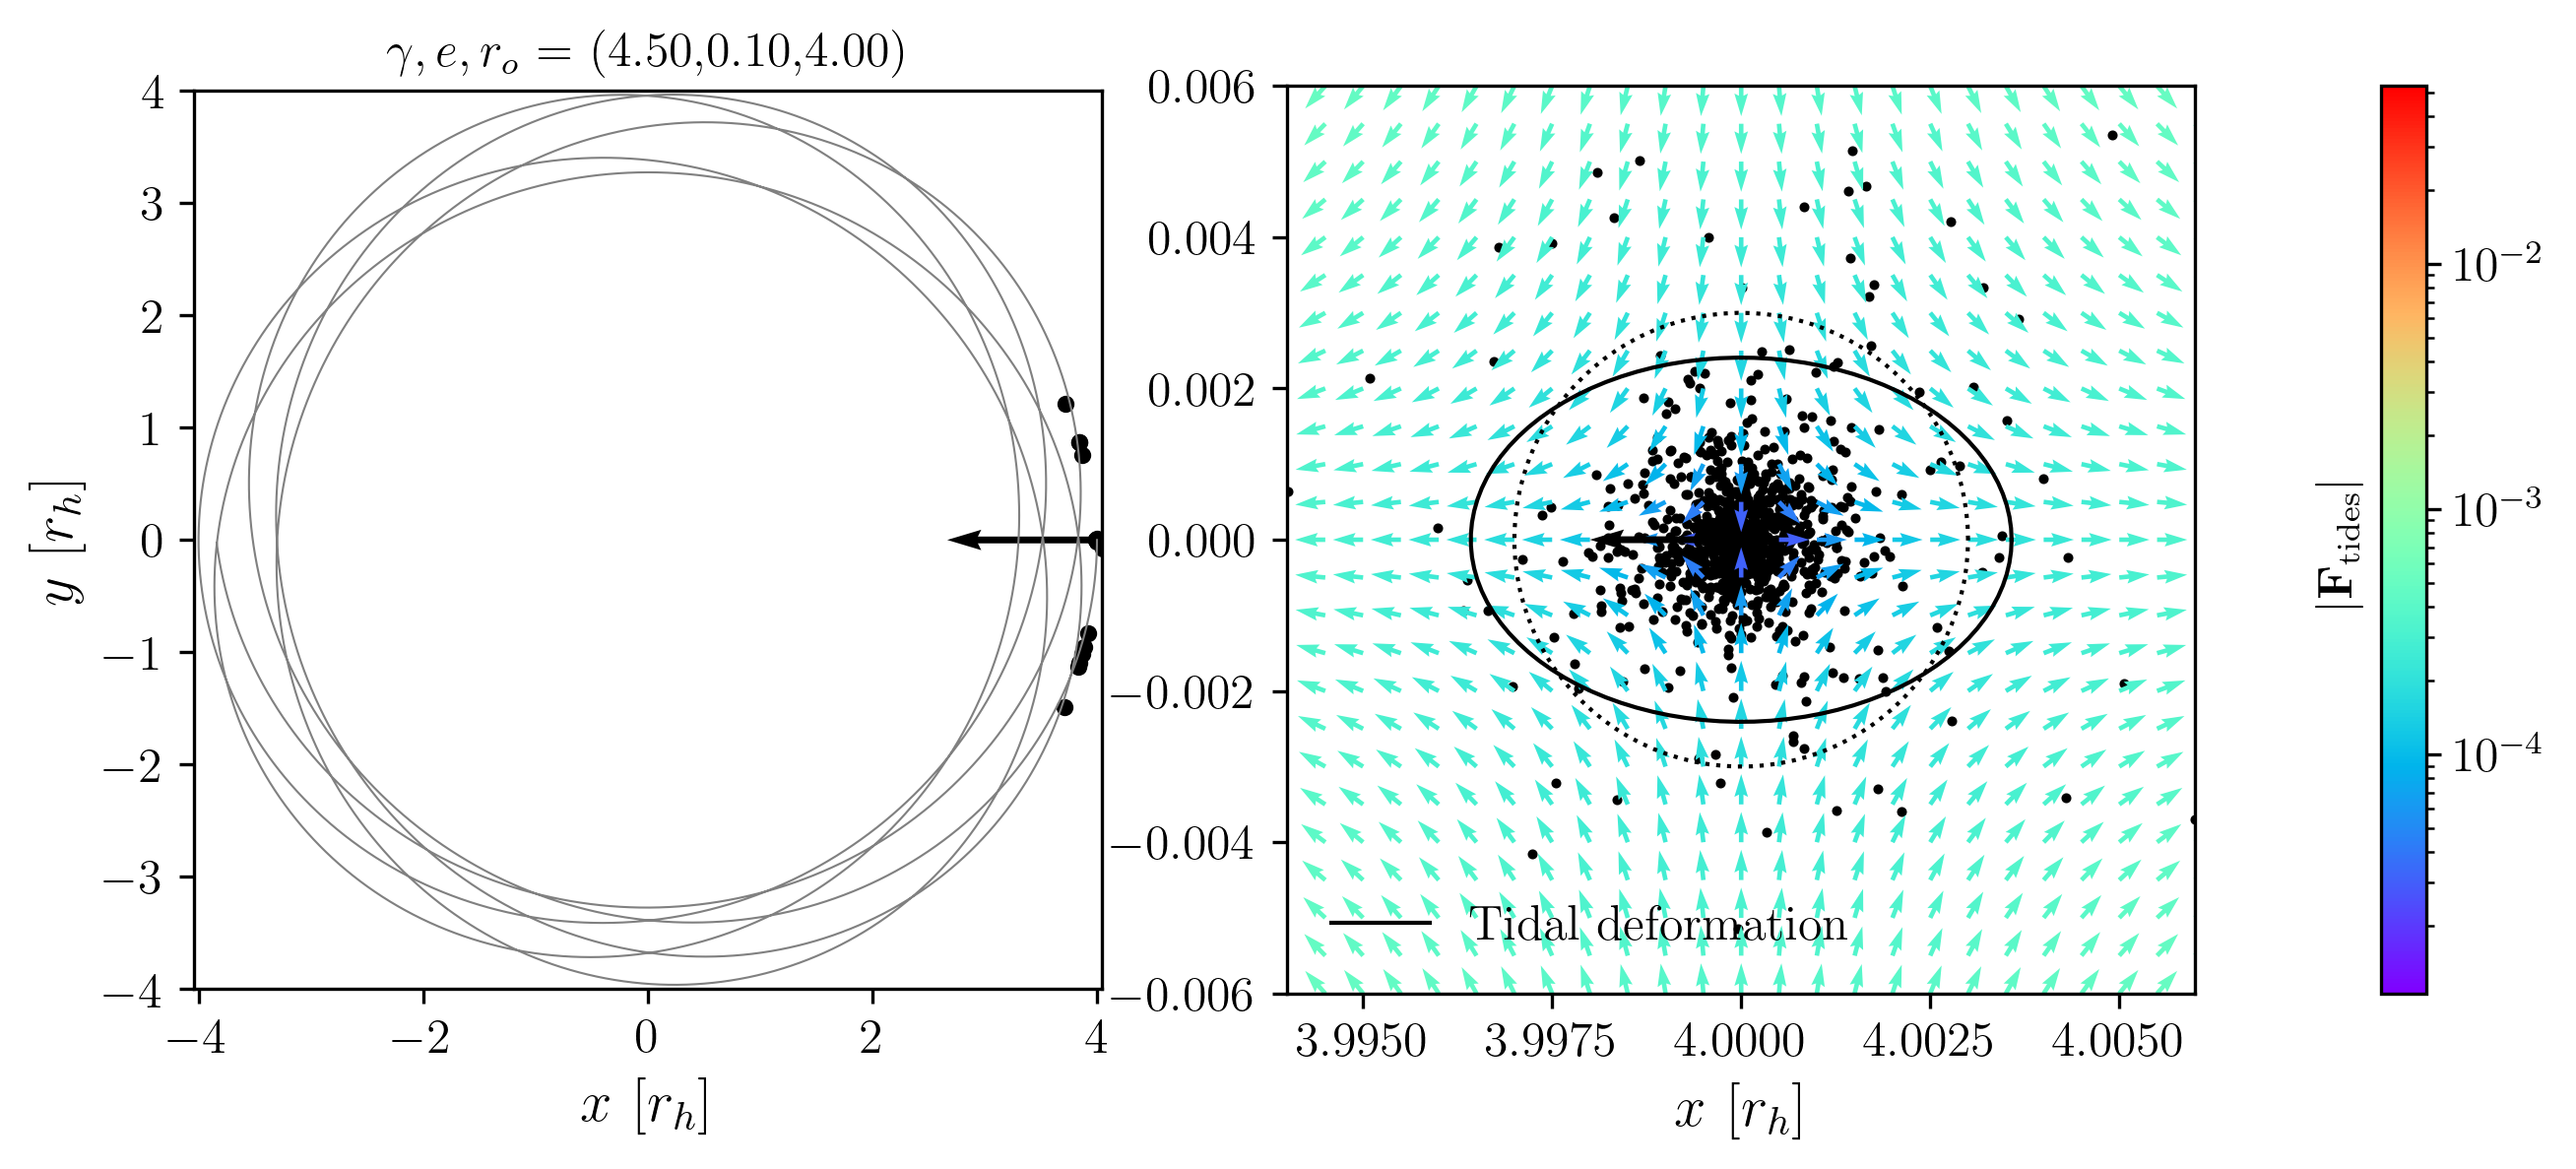
\includegraphics[width=\linewidth]{images/martos_tidal_field_450_10_400.png}
                \caption{The same experiment as Fig.~\ref{fig:martos_tidal_field_small_r}, but the cluster was placed at a larger distance of 4 $r_\textrm{halo}$, since we are beyond the characteristic radius, the tidal fields are the same, despite the different exponents $\gamma$.}
                \label{fig:martos_tidal_field_big_r}
            \end{figure}

            In the case of Fig.~\ref{fig:martos_tidal_field_big_r}, the tidal field returns to the typical situation where one axis is compressive and the other stretches. Notice how the deformations are similar in magnitude, while in the case of $\gamma=2.02$ for the top panel of Fig.~\ref{fig:martos_tidal_field_small_r}, the compression is stronger than the expansion. Both of these are different than the keplerian tidal deformation where the stronger deformation is stretching and whose axis is parallel to the position vector. 






    \subsection{Phase mixing}
        \begin{itemize}
            \item The Luiville theorem
            \item How it is slower with tidal tails 
            \item also the monte-carlo approach with phase mixing is what causes vast differences in orbital solutions after a certain period of time 
        \end{itemize}
    
    \subsection{Shocks}
        I started this section with the circular and planar restricted three body problem. It really simplifies the problem instead of looking for a general solution. All three bodies are point masses, in fact the tertiary body has no mass. The secondary is on a circular orbit about the primary, and the tertiary is in the same orbital plane as the secondary. This simplified problem is already quite complex but solvable and rich with physics. However, by restricting the orbits of the tertiary and secondary, we lose a lot of physics that affects our system. Additionally, for the globular clustres, most of them are not on circular orbits. Additionally, the galaxy is not a point mass, but rather a mass distribution with cylindrical symmetry.        



\section{The Ignored Physics}
    \subsection{Collisional dynamics}
        \begin{itemize}
            \item not nbody
            \item no mass segregation
            \item no three body encounters 
            \item no soft or hard binaries 
            \item show some results from Corespray 
        \end{itemize}
    
    \subsection{Stellar evolution}
        \begin{itemize}
            \item They're all point masses 
            \item No salpeter's 
            \item No strong initial mass loss 
            \item No accurate model for the colors 
            \item No multiple stellar populations 
        \end{itemize}
    
    \subsection{Time evolution}
        In someways, we take time evolution into account, and in someways, we ignore and this has already been covered in the previous sections. i.e., the orbit of the star-particles depend on the position of the host globular cluster, which I do not solve for simoltaneously but instead opt to load it into the computation, as shown in Section~\ref{subsec:myEquationsOfMotion}. Also, things like mass segregation and stellar evolution are time-dependent which is completely ignored in my simulations. 

